\chapter{Konzept}
In diesem Kapitel wird anhand der in Kapitel 3 erfassten Anforderungen ein Konzept entworfen. Nach der Beschreibung des Aufbaus wird der interne Ablauf, anhand von Diagrammen, detaillierter betrachtet.

\section{Aufbau der Software}
    Das in Abbildung \ref{fig:use-case} dargestellte Use-Case-Diagramm und die daraus abgeleiteten Anforderungen werden in diesem Kapitel zum Aufbau eines Konzepts verwendet.
    Hierbei wurde zunächst ein Systemdiagramm aus dem Use-Case-Diagramm abgeleitet (siehe Abbildung \ref{fig:system_all}).
    
    \begin{figure}[h]%h=direkt danach t=top b=bottom
        \centering
        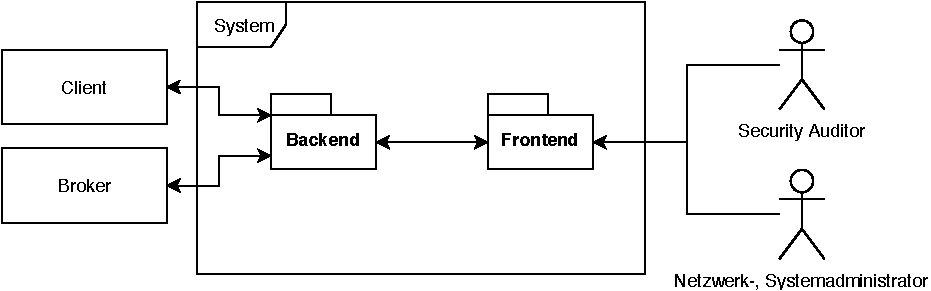
\includegraphics[width=14cm]{tex/bilder/4_konzept/Systemdiagram.pdf}
        \captionof{figure}{Systemdiagramm der Software}
        \label{fig:system_all}
    \end{figure}
    
    Die Akteure (\emph{Netzwerk-, Systemadministrator} und \emph{Security-Auditor}) konnten direkt aus dem Use-Case-Diagramm übernommen werden.
    Sie stellen die mit dem System interagierenden Nutzer dar und kommunizieren direkt mit einem Frontend.
    Es erfolgt eine klare Trennung zwischen Backend und Frontend, damit Logik und Visualisierung voneinander unabhängig implementiert werden können.
    
    Das \emph{Backend} kommuniziert durch einen Proxy mit dem Client und empfängt die gesendeten Nachrichten. Anschließend verarbeitet es diese (führt die Manipulation der Daten durch) und leitet die verarbeiteten Nachrichten an den Broker des Betreibers weiter. Sobald eine Antwort zurückkommt, wird diese erneut bearbeitet und anschließend veröffentlicht.
    Die Hauptaufgaben des Backends sind die Datenhaltung (unter anderem Speicherung der Nachrichten, Verwalten der Clients) und die Verwaltung des Nachrichtenflusses zwischen allen beteiligten Kommunikationspartnern.
    
    Das \emph{Frontend} hingegen dient nur zur Visualisierung der Nachrichten und Clients sowie zur Interaktion mit dem Nutzer. Hierbei bezieht es die gespeicherten und neu eintreffenden Nachrichten vom Backend.


    
    Abbildung \ref{fig:system_backend} zeigt eine Verfeinerung des Backends. 
    Durch das \emph{Publish/Subscribe}-Programmiermuster des \ac{MQTT}-Protokolls ist es notwendig, für jedes verbundene Gerät zwei Clients zu erzeugen, die die Nachrichten an den Betreiber übermitteln und die veröffentlichten Nachrichten wieder an den Broker des Proxys übermitteln.
    
    Einer der Clients (in diesem Fall \emph{ClientOut}) repräsentiert das tatsächliche Gerät und täuscht dies gegenüber der Endstelle des Betreiber vor. Dieser virtuelle Client übernimmt somit die Übertragung der Nachrichten zwischen dem Broker und dem Betreiber. Daraus resultiert, dass Nachrichten in gegengesetzter Richtung ebenfalls an den \emph{ClientOut} gesendet werden, auch an das physische Gerät weitergeleitet werden müssen. Dazu dient der zweite virtuelle Client (\emph{ClientIn}). Dieser erhält die vom \emph{ClientOut} erhaltene Nachricht an den Broker weiter mit der Folge, dass dieser die Nachricht anschließend veröffentlicht. Dabei muss sichergestellt werden, dass die vom Betreiber gesendete Nachricht nicht erneut nach außen gesendet wird.
    Eine grafische Darstellung des Prozesses ist Abbildung \ref{fig:aktivitaetsdiagramm_message} zu entnehmen.
    
    Der \emph{ClientManager} ermittelt die externen Clients zu den dazugehörigen \emph{ClientIn}- und \emph{ClientOut}-Instanzen. Damit wird sichergestellt, dass die Kommunikation mit dem externen Broker stattfinden kann.

    \begin{figure}[h]%h=direkt danach t=top b=bottom
        \centering
        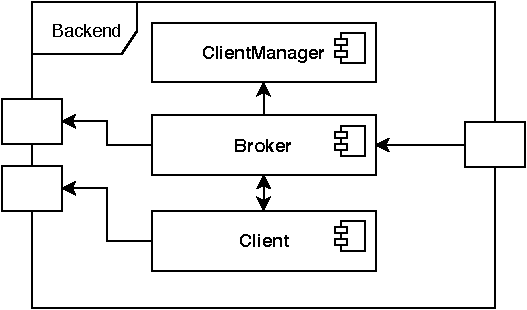
\includegraphics[width=8cm]{tex/bilder/4_konzept/Systemdiagramm_Konzept_Backend.pdf}
        \captionof{figure}{Komponentendiagramm des Backends}
        \label{fig:system_backend}
    \end{figure}
    
    Abbildung \ref{fig:system_frontend} stellt die Komponenten des Frontends dar. Alle drei Komponenten sind voneinander unabhängig und arbeiten mit unabhängigen Informationen.
    
    Die \emph{Clients}-Komponente enthält die Informationen der virtuellen Clients (\emph{ClientIn} und \emph{ClientOut}). Diese werden, sobald der Nutzer die Seite besucht, vom Backend geladen und anschließend angezeigt. Sie ermöglicht ebenfalls die Konfiguration der abzufangenden Kommunikation pro Gerät.
    
    Die \emph{NewMessages}-Komponente ermöglicht das Erzeugen von neuen Nachrichten auf der Seite des Frontends und überträgt auf Knopfdruck alle Informationen an das Backend, wo diese weiter verarbeitet (z.B. versendet) werden.
    
    Der \emph{Interceptor} ist für die Anzeige der abgefangen Nachrichten zuständig. Zu Beginn werden alle bestehenden Nachrichten abgefangen und, um das wiederholte Laden der Webseite zu verhindern und die Aktualität der Inhalte zu gewährleisten, dynamisch alle weiteren eingehenden Nachrichten nachgeladen. Um die Anzeige noch weiter strukturieren zu können, werden verschiedene Filter zur Verfügung gestellt, welche auf die Nachrichteninhalte und -attribute angewendet werden können.
    
    \begin{figure}[h]%h=direkt danach t=top b=bottom
        \centering
        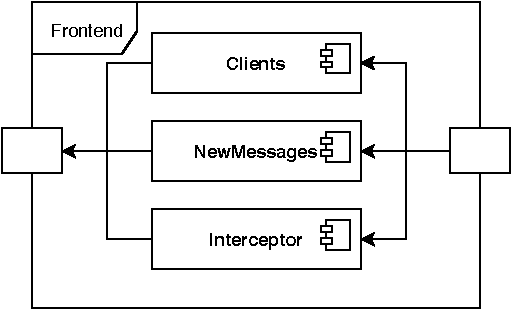
\includegraphics[width=8cm]{tex/bilder/4_konzept/Systemdiagramm_Konzept_Frontend.pdf}
        \captionof{figure}{Komponentendiagramm des Frontends}
        \label{fig:system_frontend}
    \end{figure}

\section{Prozess}
    Im Folgenden wird der interne Ablauf des zu entwickelnden Systems (auch Proxy genannt), bestehend aus dem darin enthaltenen Broker, \emph{ClientIn} und \emph{ClientOut}, beschrieben.

    Das Aktivitätsdiagramm \ref{fig:aktivitaetsdiagramm_connect} veranschaulicht den Ablauf des Verbindungsprozesses nach der Verbindungsanfrage des Clients und terminiert mit dem erfolgreichen Verbindungsaufbau.
    Sobald ein \ac{IoT}-Gerät eine Verbindung zum Proxy-Backend aufbaut, wird ein \emph{ClientManager} mit zwei virtuelle Clients (\emph{ClientOut} und \emph{ClientIn}) erzeugt. Dieser befindet sich im Proxy und steuert die Kommunikation der virtuellen Clients mit dem Broker des Betreibers. Es existiert pro physischem \ac{IoT}-Gerät nur ein \emph{ClientManager} und für den Fall, dass sich ein virtueller Client verbindet, wird die Verbindung initiiert oder erneut aufgebaut, da anzunehmen ist, dass die Verbindung unterbrochen wurde.
    
    \begin{figure}[!h]%h=direkt danach t=top b=bottom
        \centering
        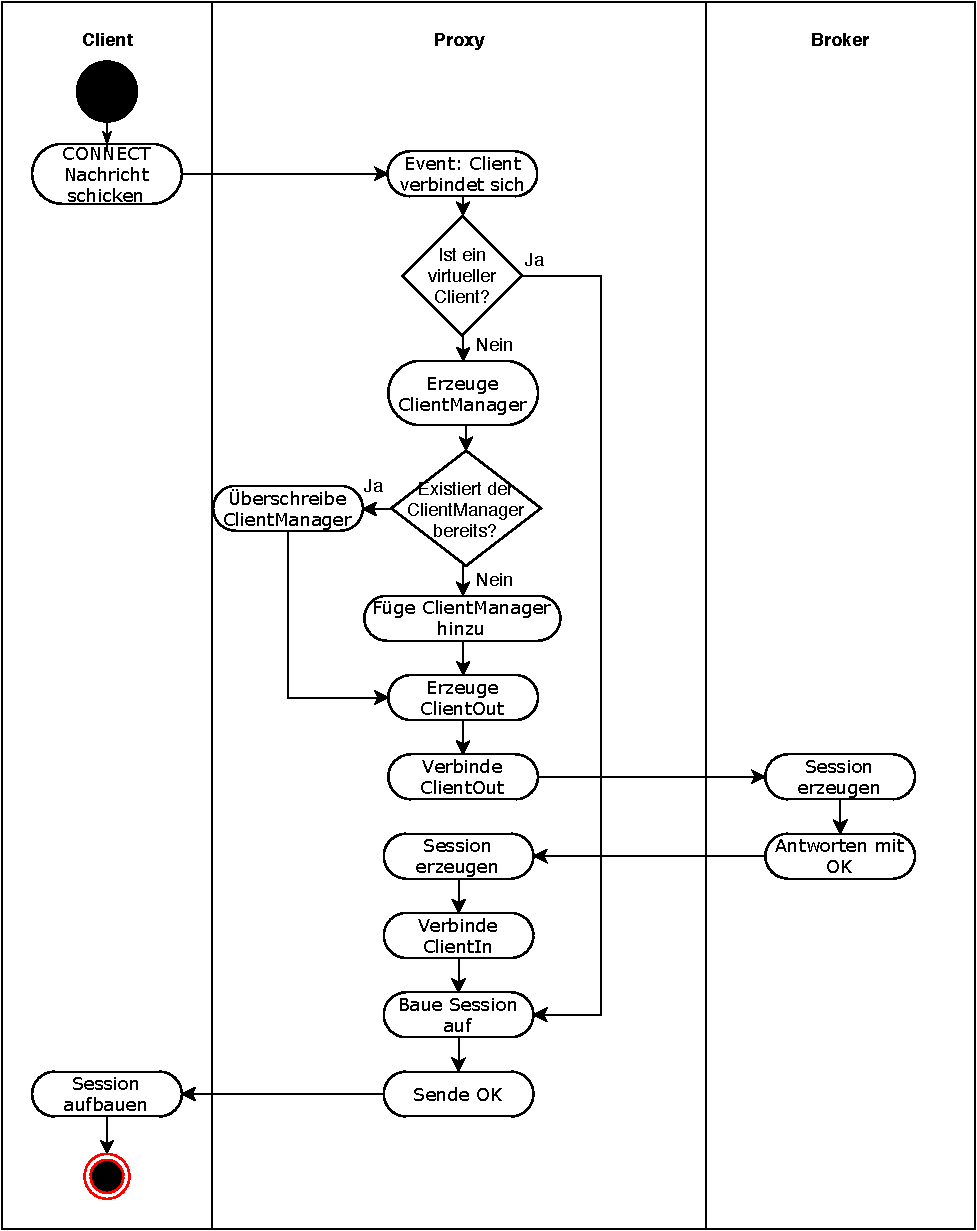
\includegraphics[width=14cm]{tex/bilder/4_konzept/Activity_Connect.pdf}
        \captionof{figure}{Aktivitätsdiagramm für das Event \emph{Client verbindet sich}}
        \label{fig:aktivitaetsdiagramm_connect}
    \end{figure}
    %%%%%%%%%%%%%%%%%%%%%%%%
    \newpage
    %%%%%%%%%%%%%%%%%%%%%%%%
    Das nächste Diagramm (\ref{fig:aktivitaetsdiagramm_message}) stellt den Nachrichtenempfangsprozess im Proxy dar.
    Durch das Event \emph{Nachricht empfangen} wird geprüft, ob die eingehende Nachricht von einem virtuellen Client kommt. Ist dies der Fall, wird diese veröffentlicht und somit dem physischen Gerät bereitgestellt. Falls nicht, wird die Veröffentlichung verhindert und abhängig von der Einstellung zum Abfangen der Nachrichten an den externen Broker weitergeleitet.
    
    \begin{figure}[!h]%h=direkt danach t=top b=bottom
        \centering
        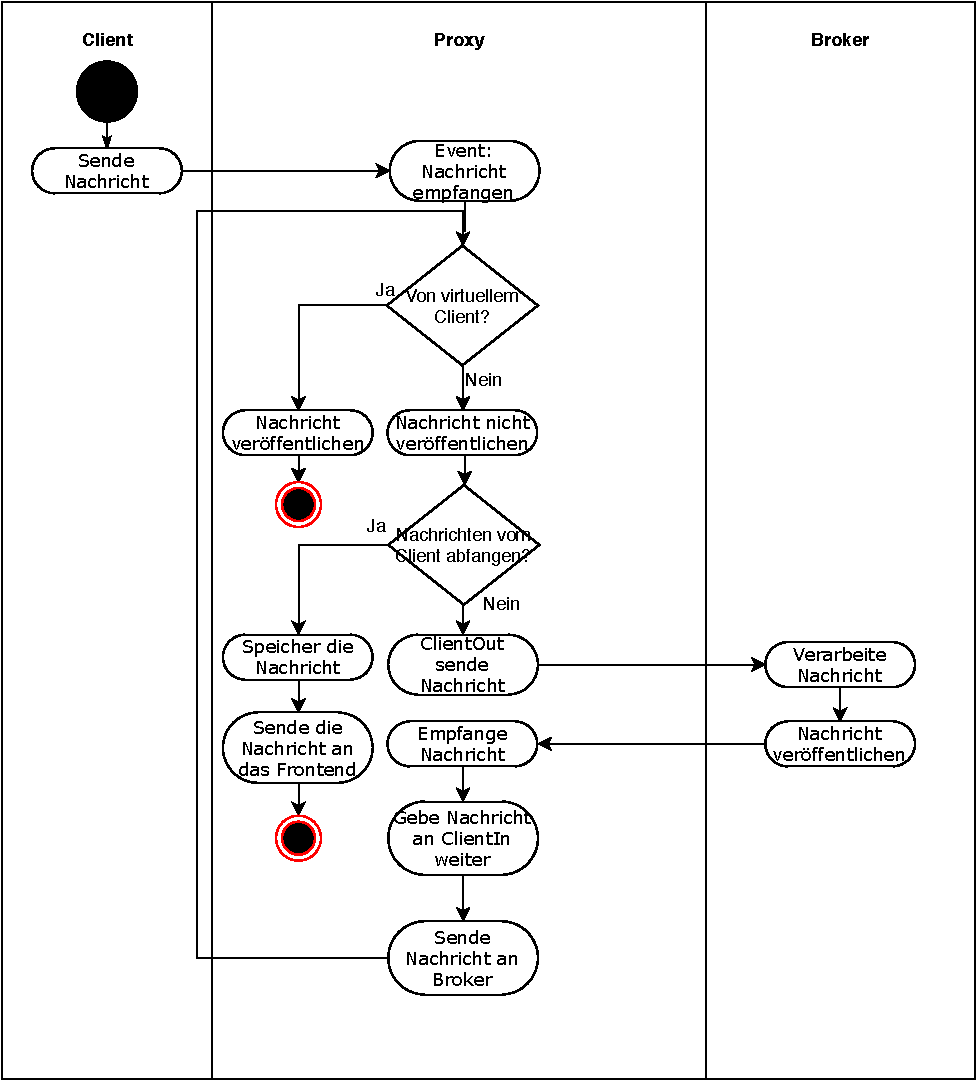
\includegraphics[width=14cm]{tex/bilder/4_konzept/Activity_Message.pdf}
        \captionof{figure}{Aktivitätsdiagramm für das Event \emph{Nachricht erhalten}}
        \label{fig:aktivitaetsdiagramm_message}
    \end{figure}
    
    Das Sequenzdiagramm (\ref{fig:sequenzdiagramm}) gibt einen detaillierten Überblick über die Kommunikation der verschiedenen Objekte und deren Interaktionen miteinander.
    Zu beachten ist, dass der Broker auf der linken Seite sowie beide virtuelle Clients Komponenten der zu entwickelnden Software (des Proxys) sind.
    Der Client sowie der Broker auf der rechten Seite repräsentieren externe Geräte, welche sich unter Umständen nicht in dem gleichen Netzwerk befinden und unabhängig vom Proxy arbeiten.
    
    \begin{figure}[!h]%h=direkt danach t=top b=bottom
        \centering
        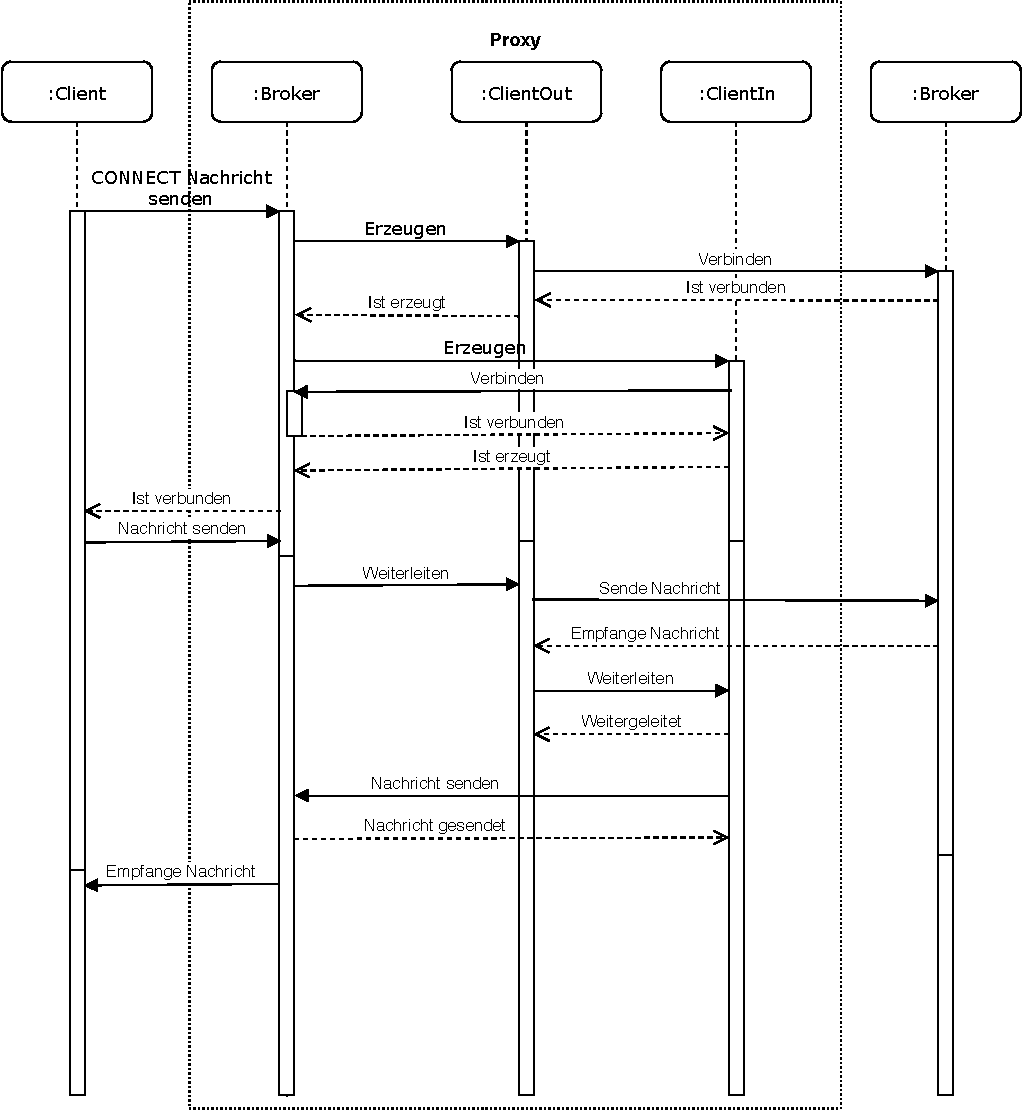
\includegraphics[width=14cm]{tex/bilder/4_konzept/Sequenz.pdf}
        \captionof{figure}{Sequenzdiagramm für die Kommunikation der Komponenten}
        \label{fig:sequenzdiagramm}
    \end{figure}

\subsubsection{Zusammenfassung}
    Ergebnis des Kapitels ist die Umsetzung der Anforderungen in eine konzeptionelle abstrakte Softwarearchitektur. Hierbei wurden die statische und Laufzeitsicht dargestellt, was als Blaupause für künftige Implementierungen dienen kann. Das Konzept lässt sich in Punkten Programmiersprache, Plattform und Protokoll große Freiheiten. Im Gegensatz dazu legt es klare Vorgaben für die Implementierungen des Proxys fest.